\documentclass{article}

  % packages
    % basic stuff for rendering math
    \usepackage[letterpaper, top=1in, bottom=1in, left=1in, right=1in]{geometry}
    \usepackage[utf8]{inputenc}
    \usepackage[english]{babel}
    \usepackage{amsmath} 
    \usepackage{amssymb}

    % extra math symbols and utilities
    \usepackage{mathtools}        % for extra stuff like \coloneqq
    \usepackage{mathrsfs}         % for extra stuff like \mathsrc{}
    \usepackage{centernot}        % for the centernot arrow 
    \usepackage{bm}               % for better boldsymbol/mathbf 
    \usepackage{enumitem}         % better control over enumerate, itemize
    \usepackage{hyperref}         % for hypertext linking
    \usepackage{fancyvrb}          % for better verbatim environments
    \usepackage{newverbs}         % for texttt{}
    \usepackage{xcolor}           % for colored text 
    \usepackage{listings}         % to include code
    \usepackage{lstautogobble}    % helper package for code
    \usepackage{parcolumns}       % for side by side columns for two column code
    

    % page layout
    \usepackage{fancyhdr}         % for headers and footers 
    \usepackage{lastpage}         % to include last page number in footer 
    \usepackage{parskip}          % for no indentation and space between paragraphs    
    \usepackage[T1]{fontenc}      % to include \textbackslash
    \usepackage{footnote}
    \usepackage{etoolbox}

    % for custom environments
    \usepackage{tcolorbox}        % for better colored boxes in custom environments
    \tcbuselibrary{breakable}     % to allow tcolorboxes to break across pages

    % figures
    \usepackage{pgfplots}
    \pgfplotsset{compat=1.18}
    \usepackage{float}            % for [H] figure placement
    \usepackage{tikz}
    \usepackage{tikz-cd}
    \usepackage{circuitikz}
    \usetikzlibrary{arrows}
    \usetikzlibrary{positioning}
    \usetikzlibrary{calc}
    \usepackage{graphicx}
    \usepackage{algorithmic}
    \usepackage{caption} 
    \usepackage{subcaption}
    \captionsetup{font=small}

    % for tabular stuff 
    \usepackage{dcolumn}

    \usepackage[nottoc]{tocbibind}
    \pdfsuppresswarningpagegroup=1
    \hfuzz=5.002pt                % ignore overfull hbox badness warnings below this limit

  % New and replaced operators
    \DeclareMathOperator{\Tr}{Tr}
    \DeclareMathOperator{\Sym}{Sym}
    \DeclareMathOperator{\Span}{span}
    \DeclareMathOperator{\std}{std}
    \DeclareMathOperator{\Cov}{Cov}
    \DeclareMathOperator{\Var}{Var}
    \DeclareMathOperator{\Corr}{Corr}
    \DeclareMathOperator{\pos}{pos}
    \DeclareMathOperator*{\argmin}{\arg\!\min}
    \DeclareMathOperator*{\argmax}{\arg\!\max}
    \newcommand{\ket}[1]{\ensuremath{\left|#1\right\rangle}}
    \newcommand{\bra}[1]{\ensuremath{\left\langle#1\right|}}
    \newcommand{\braket}[2]{\langle #1 | #2 \rangle}
    \newcommand{\qed}{\hfill$\blacksquare$}     % I like QED squares to be black

  % Custom Environments
    \newtcolorbox[auto counter, number within=section]{question}[1][]
    {
      colframe = orange!25,
      colback  = orange!10,
      coltitle = orange!20!black,  
      breakable, 
      title = \textbf{Question \thetcbcounter ~(#1)}
    }

    \newtcolorbox[auto counter, number within=section]{exercise}[1][]
    {
      colframe = teal!25,
      colback  = teal!10,
      coltitle = teal!20!black,  
      breakable, 
      title = \textbf{Exercise \thetcbcounter ~(#1)}
    }
    \newtcolorbox[auto counter, number within=section]{solution}[1][]
    {
      colframe = violet!25,
      colback  = violet!10,
      coltitle = violet!20!black,  
      breakable, 
      title = \textbf{Solution \thetcbcounter}
    }
    \newtcolorbox[auto counter, number within=section]{lemma}[1][]
    {
      colframe = red!25,
      colback  = red!10,
      coltitle = red!20!black,  
      breakable, 
      title = \textbf{Lemma \thetcbcounter ~(#1)}
    }
    \newtcolorbox[auto counter, number within=section]{theorem}[1][]
    {
      colframe = red!25,
      colback  = red!10,
      coltitle = red!20!black,  
      breakable, 
      title = \textbf{Theorem \thetcbcounter ~(#1)}
    } 
    \newtcolorbox[auto counter, number within=section]{proposition}[1][]
    {
      colframe = red!25,
      colback  = red!10,
      coltitle = red!20!black,  
      breakable, 
      title = \textbf{Proposition \thetcbcounter ~(#1)}
    } 
    \newtcolorbox[auto counter, number within=section]{corollary}[1][]
    {
      colframe = red!25,
      colback  = red!10,
      coltitle = red!20!black,  
      breakable, 
      title = \textbf{Corollary \thetcbcounter ~(#1)}
    } 
    \newtcolorbox[auto counter, number within=section]{proof}[1][]
    {
      colframe = orange!25,
      colback  = orange!10,
      coltitle = orange!20!black,  
      breakable, 
      title = \textbf{Proof. }
    } 
    \newtcolorbox[auto counter, number within=section]{definition}[1][]
    {
      colframe = yellow!25,
      colback  = yellow!10,
      coltitle = yellow!20!black,  
      breakable, 
      title = \textbf{Definition \thetcbcounter ~(#1)}
    } 
    \newtcolorbox[auto counter, number within=section]{example}[1][]
    {
      colframe = blue!25,
      colback  = blue!10,
      coltitle = blue!20!black,  
      breakable, 
      title = \textbf{Example \thetcbcounter ~(#1)}
    } 
    \newtcolorbox[auto counter, number within=section]{code}[1][]
    {
      colframe = green!25,
      colback  = green!10,
      coltitle = green!20!black,  
      breakable, 
      title = \textbf{Code \thetcbcounter ~(#1)}
    } 
    \newtcolorbox[auto counter, number within=section]{algo}[1][]
    {
      colframe = green!25,
      colback  = green!10,
      coltitle = green!20!black,  
      breakable, 
      title = \textbf{Algorithm \thetcbcounter ~(#1)}
    } 

    \definecolor{dkgreen}{rgb}{0,0.6,0}
    \definecolor{gray}{rgb}{0.5,0.5,0.5}
    \definecolor{mauve}{rgb}{0.58,0,0.82}
    \definecolor{darkblue}{rgb}{0,0,139}
    \definecolor{lightgray}{gray}{0.93}
    \renewcommand{\algorithmiccomment}[1]{\hfill$\triangleright$\textcolor{blue}{#1}}

    % default options for listings (for code)
    \lstset{
      autogobble,
      frame=ltbr,
      language=Python,
      aboveskip=3mm,
      belowskip=3mm,
      showstringspaces=false,
      columns=fullflexible,
      keepspaces=true,
      basicstyle={\small\ttfamily},
      numbers=left,
      firstnumber=1,                        % start line number at 1
      numberstyle=\tiny\color{gray},
      keywordstyle=\color{blue},
      commentstyle=\color{dkgreen},
      stringstyle=\color{mauve},
      backgroundcolor=\color{lightgray}, 
      breaklines=true,                      % break lines
      breakatwhitespace=true,
      tabsize=3, 
      xleftmargin=2em, 
      framexleftmargin=1.5em, 
      stepnumber=1
    }

  % Page style
    \pagestyle{fancy}
    \fancyhead[L]{}
    \fancyhead[C]{Muchang Bahng}
    \fancyhead[R]{Spring 2025} 
    \fancyfoot[C]{\thepage / \pageref{LastPage}}
    \renewcommand{\footrulewidth}{0.4pt}          % the footer line should be 0.4pt wide
    \renewcommand{\thispagestyle}[1]{}  % needed to include headers in title page

\begin{document}

\title{Networks}
\author{Muchang Bahng}
\date{Spring 2025}

\maketitle
\tableofcontents
\pagebreak

\section{Networking} 

  Networking is a large field in itself, but in here I go over the most useful and practical applications of it in my everyday use. Some ways that I personally benefit from this is:

  \begin{enumerate}
    \item Connecting to WiFi and diagnosing problems.  
    \item Connecting to WiFi and diagnosing problems. 
    \item Connecting to other networks such as computing clusters or third-party blockchains.  
    \item Seeing how more abstract schemes such as APIs work. 
    \item Ethical hacking. 
  \end{enumerate}
  I introduce these concepts and how to do some basic implementation a Unix operating system.

  I like to learn about networking as if I am designing it from scratch. Some big questions to ask when designing network schemes are:

  \begin{enumerate}
    \item How do we uniquely identify computers? 
    \item How should we establish a connection between them? Through hardware or signals? 
    \item What protocols should we use, like a common language, so that all computers understand what each other are saying? 
    \item Can we implement security measures to prevent unwanted visitors into our computer? 
  \end{enumerate} 

  \subsection{Computer Networks and the Internet}

    Let us first define a computer network, some of its architecture, and then move onto the Internet. 

    \begin{definition}[Computer Network]
      A \textbf{computer network} is a group of computers (i.e. computing devices) that use a set of common \textit{communication protocols} over digital interconnections for the purpose of sharing resources located on or provided by the \textit{network nodes}, which may include personal computers, servers, networking hardware, or other specialised or general-purpose hosts. 

    \end{definition}

    These network nodes may be able to communicate to certain neighboring nodes, and this graph architecture determines the \textbf{network topology}. A computer network can be visualized as a connected graph of nodes 

    \begin{example}[Network Topologies]
      Common layouts are: 

      \begin{enumerate}
        \item \textbf{Line Network}: All nodes are connected in a line. 

        \begin{center}\resizebox{8cm}{0.64cm}{%
        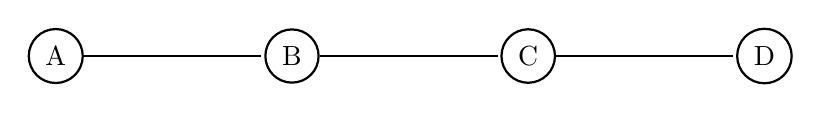
\begin{tikzpicture}[-,>=stealth',shorten >=1pt,auto,node distance=3cm, thick,main node/.style={circle,draw}, every loop/.style={}, scale=0.7]
            \node[main node] (A) {A};
            \node[main node] (B) [right of=A] {B};
            \node[main node] (C) [right of=B] {C};
            \node[main node] (D) [right of=C] {D};
            \path[every node/.style={font=\sffamily\small}]
            (A) edge node {} (B)
            (B) edge node {} (C)
            (C) edge node {} (D);
        \end{tikzpicture}}
        \end{center}

          \item \textbf{Bus Network}: All nodes are connected to a common medium along this medium. 

        \item \textbf{Star Network}: all nodes are connected to a special central node.
          \begin{center}
          \resizebox{3cm}{3cm}{%
          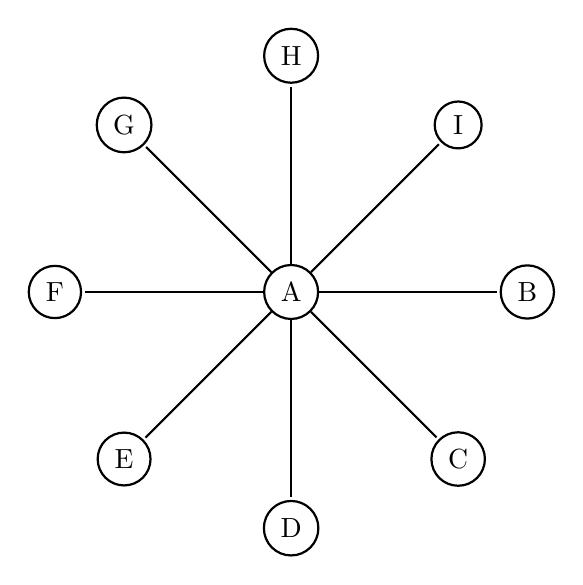
\begin{tikzpicture}[-,>=stealth',shorten >=1pt,auto,node distance=3cm, thick,main node/.style={circle,draw}, every loop/.style={}]
              \node[main node] (A) {A};
              \node[main node] (B) [right of=A] {B};
              \node[main node] (C) [below right of=A] {C};
              \node[main node] (D) [below of=A] {D};
              \node[main node] (E) [below left of=A] {E};
              \node[main node] (F) [left of=A] {F};
              \node[main node] (G) [above left of=A] {G};
              \node[main node] (H) [above of=A] {H};
              \node[main node] (I) [above right of=A] {I};
              \path[every node/.style={font=\sffamily\small}]
              (A) edge node {} (B)
              (A) edge node {} (C)
              (A) edge node {} (D)
              (A) edge node {} (E)
              (A) edge node {} (F)
              (A) edge node {} (G)
              (A) edge node {} (H)
              (A) edge node {} (I);
          \end{tikzpicture}}
          \end{center}

        \item \textbf{Ring Network}: Each node is connected to its left and right neighbour node, such that all nodes are connected and that each node can reach each other node by traversing nodes left- or rightwards.
          \begin{center}
          \resizebox{3cm}{3cm}{%
          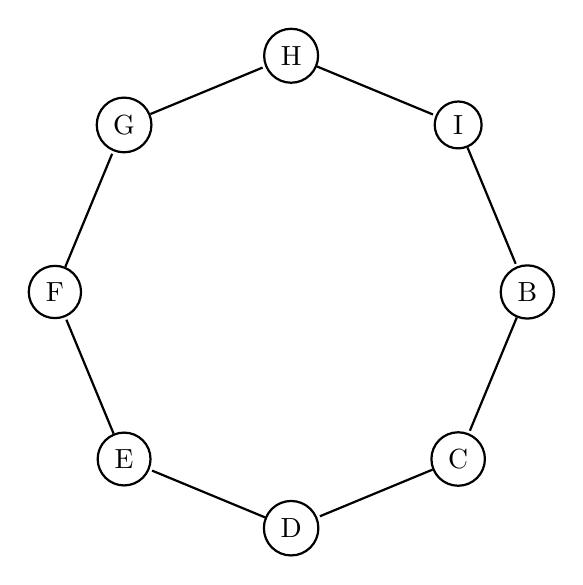
\begin{tikzpicture}[-,>=stealth',shorten >=1pt,auto,node distance=3cm, thick,main node/.style={circle,draw}, every loop/.style={}]
              \node[main node] (A) {A};
              \draw[white, fill=white] (-1,-1) rectangle (1,1);
              \node[main node] (B) [right of=A] {B};
              \node[main node] (C) [below right of=A] {C};
              \node[main node] (D) [below of=A] {D};
              \node[main node] (E) [below left of=A] {E};
              \node[main node] (F) [left of=A] {F};
              \node[main node] (G) [above left of=A] {G};
              \node[main node] (H) [above of=A] {H};
              \node[main node] (I) [above right of=A] {I};
              \path[every node/.style={font=\sffamily\small}]
              (B) edge node {} (C)
              (C) edge node {} (D)
              (D) edge node {} (E)
              (E) edge node {} (F)
              (F) edge node {} (G)
              (G) edge node {} (H)
              (H) edge node {} (I)
              (I) edge node {} (B);
          \end{tikzpicture}}
          \end{center}

        \item \textbf{Mesh Network}: each node is connected to an arbitrary number of neighbours in such a way that there is at least one traversal from any node to any other. 
          \begin{center}
          \resizebox{3.5cm}{3cm}{%
          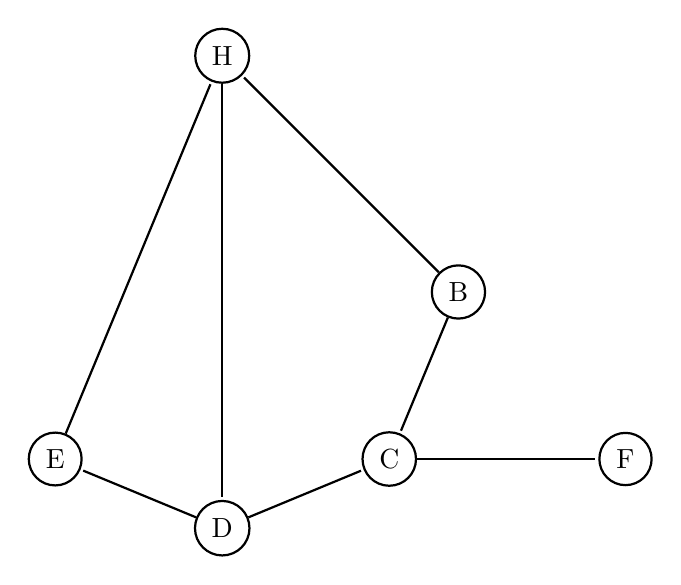
\begin{tikzpicture}[-,>=stealth',shorten >=1pt,auto,node distance=3cm, thick,main node/.style={circle,draw}, every loop/.style={}]
              \node[main node] (A) {A};
              \draw[white, fill=white] (-1,-1) rectangle (1,1);
              \node[main node] (B) [right of=A] {B};
              \node[main node] (C) [below right of=A] {C};
              \node[main node] (D) [below of=A] {D};
              \node[main node] (E) [below left of=A] {E};
              \node[main node] (H) [above of=A] {H};
              \node[main node] (F) [right of=C] {F};
              \path[every node/.style={font=\sffamily\small}]
              (B) edge node {} (C)
              (B) edge node {} (H)
              (D) edge node {} (C)
              (D) edge node {} (E)
              (C) edge node {} (F)
              (E) edge node {} (H)
              (H) edge node {} (D);
          \end{tikzpicture}}
          \end{center}

        \item \textbf{Fully Connected Network}: each node is connected to every other node in the network.
          \begin{center}
          \resizebox{3cm}{3cm}{%
          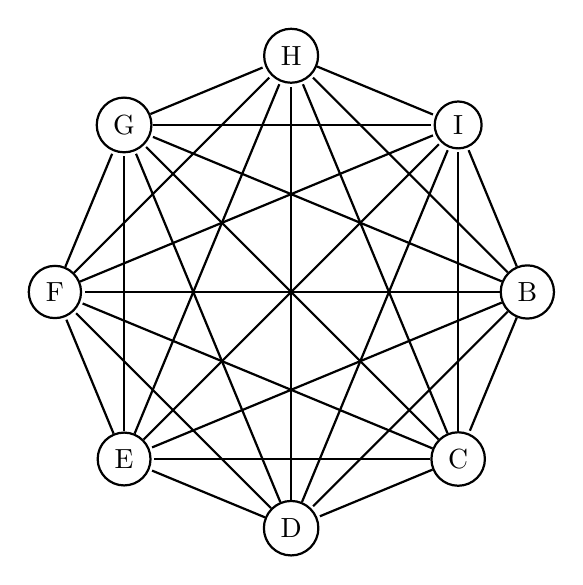
\begin{tikzpicture}[-,>=stealth',shorten >=1pt,auto,node distance=3cm, thick,main node/.style={circle,draw}, every loop/.style={}]
              \node[main node] (A) {A};
              \draw[white, fill=white] (-1,-1) rectangle (1,1);
              \node[main node] (B) [right of=A] {B};
              \node[main node] (C) [below right of=A] {C};
              \node[main node] (D) [below of=A] {D};
              \node[main node] (E) [below left of=A] {E};
              \node[main node] (F) [left of=A] {F};
              \node[main node] (G) [above left of=A] {G};
              \node[main node] (H) [above of=A] {H};
              \node[main node] (I) [above right of=A] {I};
              \path[every node/.style={font=\sffamily\small}]
              (B) edge node {} (C)
              (B) edge node {} (D)
              (B) edge node {} (E)
              (B) edge node {} (F)
              (B) edge node {} (G)
              (B) edge node {} (H)
              (B) edge node {} (I)
              (C) edge node {} (D)
              (C) edge node {} (E)
              (C) edge node {} (F)
              (C) edge node {} (G)
              (C) edge node {} (H)
              (C) edge node {} (I)
              (D) edge node {} (E)
              (D) edge node {} (F)
              (D) edge node {} (G)
              (D) edge node {} (H)
              (D) edge node {} (I)
              (E) edge node {} (F)
              (E) edge node {} (G)
              (E) edge node {} (H)
              (E) edge node {} (I)
              (F) edge node {} (G)
              (F) edge node {} (H)
              (F) edge node {} (I)
              (G) edge node {} (H)
              (G) edge node {} (I)
              (H) edge node {} (I);
          \end{tikzpicture}}
          \end{center}

        \item \textbf{Tree Network}: nodes are arranged hierarchically.
          \begin{center}
          \resizebox{5cm}{3cm}{%
          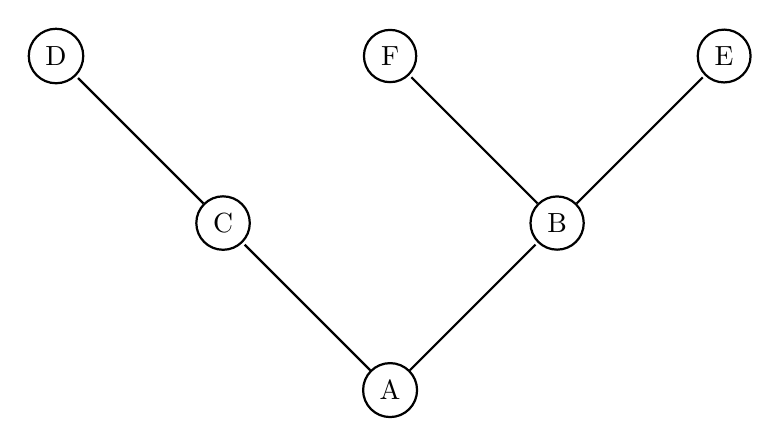
\begin{tikzpicture}[-,>=stealth',shorten >=1pt,auto,node distance=3cm, thick,main node/.style={circle,draw}, every loop/.style={}]
              \node[main node] (A) {A};
              \node[main node] (B) [above right of=A] {B};
              \node[main node] (C) [above left of=A] {C};
              \node[main node] (D) [above left of=C] {D};
              \node[main node] (E) [above right of=B] {E};
              \node[main node] (F) [above left of=B] {F};
              \path[every node/.style={font=\sffamily\small}]
              (A) edge node {} (B)
              (A) edge node {} (C)
              (B) edge node {} (F)
              (B) edge node {} (E)
              (C) edge node {} (D);
          \end{tikzpicture}}
          \end{center}
      \end{enumerate} 
    \end{example}

    Notice how many of these networks have \textbf{redundancy}: having multiple ways to get from one node to another. That is, when a network path is no longer available, data is still able to reach its destination through another path. Usually, we would like to avoid a \textbf{single point of failure} and construct a \textbf{fault-tolerant} system that can experience failure in its components but still continue operating properly. However, building more connections may be expensive. 

    Because there are multiple paths that a piece of data takes to get from point X to point Y, \textit{routing strategies} are implemented in order to determine the most optimal path. Now in order for network nodes to communicate with each other, they should have some sort of universal method of communicating with each other. 

    \begin{definition}[Communication Protocol]
      A \textbf{communication protocol} is a system of rules that allow multiple entities of a communications to transmit information via any kind variation of a physical quantity. The protocol defines the rules, syntax, semantics and synchronization of communication and possible error recovery methods. A protocol can have many jobs, such as: 
      
      \begin{enumerate} 
        \item Determining how nodes will communicate with each other . 
        \item Making sure that these modes of communication is compatible with hardware .
        \item Implementing security protocols such as encryption schemes. 
      \end{enumerate}
    \end{definition}

    Computers can connect through \textbf{physical} (e.g. cables) or \textbf{wireless} connections. 

    \begin{enumerate}
      \item The \textbf{CAT5 cable} is a \textit{twisted pair (copper) cable} that's designed for use in computer networks. It consists of four twisted pairs of copper wires. These twisted pair cables send data through a network by transmitting pulses of electricity that represent binary data. The information transmission follow the \textbf{Ethernet} standards, which is why twisted pair cables are commonly known as Ethernet cables. Use for both LANs and WANs. They can carry up to 1 Gbps across hundreds of feet, but are susceptible to interference. 

      \item \textbf{Fiber-optic cables} carry light instead of electricity in a fiber coated with plastic layers. The pulses of light represent binary data and also follow the Ethernet standards. They are also capable of transmitting much more data per second that copper cables, and they have the advantage of low transmission loss and immunity to electrical interference. Often used to connect networks across oceans so that data can travel quickly around the world. They can carry up to 26 Tbps acorss 50 miles (but are expensive)

      \item A wireless card inside a computer turns binary data into \textbf{radio waves} and transmits them through the air. However, they do not travel very far (~100 ft in office buildings or up to 1000 ft in an open field). The waves are picked up by a \textit{wireless access point} which converts them from radio waves back into binary data. These access points would be connected to the rest of the network using physical wiring. They can carry up to 1.3 Gbps. 

      \item \textbf{Infrared signals} and \textbf{microwaves} are sometimes used. 
    \end{enumerate}


    In order for the computers to send data into binary, they must convert this data into binary and send them as streams of 1s and 0s in a process called \textbf{line coding}. Furthermore, computers can raise efficiency of each wire by sending changing electric currents through a single wire. For example, rather than using three wires to encode $\texttt{101}$ as 

    \begin{center}
      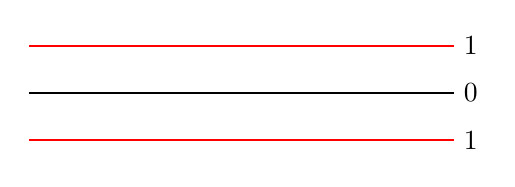
\begin{tikzpicture}[scale=0.6]
        \draw[thick, red] (0,1)--(9,1);
        \draw[thick] (0,0)--(9,0);
        \draw[thick, red] (0,-1)--(9,-1);
        \node[right] at (9,1) {1};
        \node[right] at (9,0) {0}; 
        \node[right] at (9,-1) {1};
      \end{tikzpicture}
    \end{center}

    they send it through a single wire with intervals of $\frac{1}{3}$ seconds

    \begin{center}
      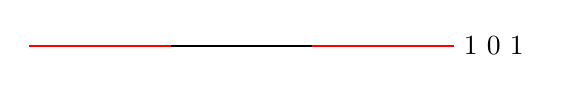
\begin{tikzpicture}[scale=0.6]
        \draw[thick, red] (0,0)--(3,0);
        \draw[thick] (3,0)--(6,0);
        \draw[thick, red] (6,0)--(9,0);
        \node[right] at (9,0) {1 0 1};
      \end{tikzpicture}
    \end{center}

    or even better, at a rate of 1 megabit per second (interval of $0.000001$ seconds)

    \begin{center}
      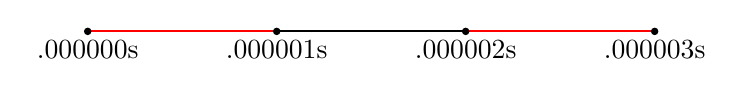
\begin{tikzpicture}[scale=0.8]
        \draw[thick, red] (0,0)--(3,0);
        \draw[thick] (3,0)--(6,0);
        \draw[thick, red] (6,0)--(9,0);
        \draw[fill] (0,0) circle (0.05);
        \draw[fill] (3,0) circle (0.05);
        \draw[fill] (6,0) circle (0.05);
        \draw[fill] (9,0) circle (0.05);
        \node[below] at (0,0) {.000000s};
        \node[below] at (3,0) {.000001s};
        \node[below] at (6,0) {.000002s};
        \node[below] at (9,0) {.000003s};
      \end{tikzpicture}
    \end{center}

    As long as two computers agree on the time period in which the electricity intervals are being sent, they can communicate much more efficiently. In an electrical connection (such as Ethernet), the signal would be a voltage or current. In an optical connection (such as a fiber-optic cable), the signal would be the intensity of light. 

    \begin{definition}
      There are many properties about line coding that are relevant, but ultimately the speed of a connection is a combination of the bandwidth and latency. 

      \begin{enumerate}
        \item The \textbf{bit rate} describes the data transfer rate of a connection. It measures the number of bit states that a channel can \textit{transmit} per unit time. It is measured in \textit{bits per second}. We can interpret it as the amount of water flowing through a pipe. 
        
        Bit rate is typically seen in terms of the actual data rate. But for most transmissions, the data represents part of a more complex protocol, which includes bits representing source address, destination address, error detection/correction codes, and other information. This data is called the \textbf{overhead}, while the actual data transferred is called the \textbf{payload}. At times, the overhead may be substantial (up to 20\% to 50\%). 

        \item The \textbf{throughput} is the number of bit states of usable information, that can be successfully \textit{received} over a channel per unit time. Without any channel noise, it is really just the payload. Note that this is an \textit{observed, dynamic parameter} with a fixed and variable loss. It is also known as \textbf{consumed bandwidth} and is measured in \textit{bits per second}. 
        
        \item The \textbf{bandwidth} describes the \textit{maximum} data transfer rate of a connection; that is, the maximum throughput of a communication. It is measured in \textit{bits per second}. We can interpret it as how thick the pipe is (i.e. how much water can flow through it at max). Note that this is different from the bandwidth used in signal processing. 
        
        Data often flows over multiple network connections, which means the connection with the smallest bandwidth (most likely your local connection) acts as a bottleneck. 
        
        \item The \textbf{latency}, or \textbf{ping-rate}, measures the round trip time between the sending of a data message to a computer and the receiving of that message, measured in \textit{milliseconds}. We can interpret it as the speed at which the water is flowing through a pipe. We can check latency by doing
        \begin{lstlisting}
          >>>ping www.google.com
          64 bytes: icmp_seq=0 ttl=115 time=37.868 ms
        \end{lstlisting}

        which outputs a latency time of 37.868ms (to get to $\texttt{www.google.com}$ and back) for sending a data packet of 64 bytes. Note that there is an intrinsic limiting factor to latency: the speed of light, which is approximately 1 foot per nanosecond. In addition to distance, another limiting factor is the congestion in the network and the type of connection. 
      \end{enumerate}
    \end{definition}

    \begin{example}
    Given two computers connected by a wire that is configured to transfer 1000 bits per second, the bit rate would be 1 Kbps. However, if the channel has noise and demands retransmission of 10 bits out of every 1000 of the original transmission, then the throughput would be 990 bps. 

    Furthermore, the Ethernet frame can have as many as 1542 bytes. Say that there are 1500 bytes of payload and an overhead of 42 bytes. Then, the \textbf{protocol efficiency} would would be 
    \[\frac{\text{payload}}{\text{frame size}} = \frac{1500}{1542} = 0.9727 = 97.3\%\]
    \end{example}

    Typically, the actual line rate is stepped up by a factor influenced by the overhead to achieve an actual target net data rate. In One Gigabit Ethernet, the actual line rate is 1.25 Gbits/s to achieve a net payload throughput of 1 Gbit/s. In a 10-Gbit/s Ethernet system, gross data rate equals 10.3125 Gbits/s to achieve a true data rate of 10 Gbits/s. The net data rate also is referred to as the throughput, or payload rate, of effective data rate.

  \subsection{History of the Internet}

    IETF, ICANN, IANA, ISPs.  

    \begin{example}[ARPANET]
      The ARPANET was the precursor to the Internet, the network where Internet technology was first tested out. It was started in 1969 with four computers connected to each other. 

        \begin{center}\resizebox{5cm}{3cm}{%
        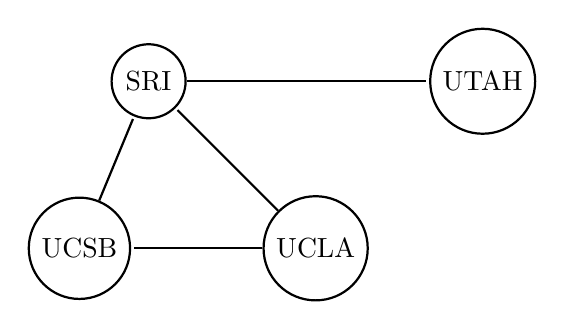
\begin{tikzpicture}[-,>=stealth',shorten >=1pt,auto,node distance=3cm, thick,main node/.style={circle,draw}, every loop/.style={}]
            \node[main node] (UCLA) {UCLA};
            \node[main node] (UCSB) [left of=UCLA] {UCSB};
            \node[main node] (SRI) [above left of=UCLA] {SRI};
            \node[main node] (UTAH) [above right of=UCLA] {UTAH};
            \path[every node/.style={font=\sffamily\small}]
            (UCLA) edge node {} (UCSB)
            (UCLA) edge node {} (SRI)
            (UCSB) edge node {} (SRI)
            (SRI) edge node {} (UTAH);
        \end{tikzpicture}}
        \end{center}

      For example, even if the path between SRI and UCSB is gone, the connections between SRI and UCSB is not lost (since IP packets can travel through UCLA's router). 
    \end{example}


    Now we can see an implementation of these networks in the internet. 

    \begin{definition}[Internet]
      The \textbf{Internet} is a global network of computing devices communicating with each other in some way, whether they're sending emails, downloading files, or sharing websites. The Internet is an \textbf{open network}, which means that any computing device can join as long as they follow the protocols. The internet is powered by many layers of protocols, and to create a global network of computing devices, we need: 

      \begin{enumerate}
        \item \textbf{Wires \& Wireless}: Physical connections between devices, plus protocols for converting electromagnetic signals into binary data. 
        \item \textbf{IP}: A protocol that uniquely identifies devices using IP addresses and provides a routing strategy to send data to a destination IP address. 
        \item \textbf{TCP/UDP}: Protocols that can transport packets of data from one device to another and check for errors along the way. 
        \item \textbf{TLS}: A secure protocol for sending encrypted data so that attackers can't view private information. 
        \item \textbf{HTTP \& DNS}: The protocols powering the World Wide Web
      \end{enumerate}        
    \end{definition}

    An \textbf{ISP (Internet Service Provider)} provides internet to its region. These ISPs are managed by certain continental autonomous systems (\textbf{AS}). The \textbf{Regional Internet Registry (RIR)} is divided into their regions: AFRNIC (Africa), ARIN (American), APNIC (Asia-Pacific), LACNIC (Latin America and Carribean), and RIPE NCC (European). 

    The main protocol suite used by the internet is \textbf{TCP/IP}, which is a collection of protocols that the internet uses. The bulk of this chapter will describe this protocol. 

    \begin{figure}[hbt!]
      \centering
      \includegraphics[scale=0.7]{img/tcp_ip_model.png}
      \caption{TCP/IP layering model. }
      \label{fig:tcp_ip_model}
    \end{figure}

  \subsection{Network Interfaces}

    Before we even start talking about IP addresses or protocols, we should mention that there are several interfaces from which computers can send and receive data. For example, if you are connected to both wired ethernet and WiFi, there are two paths, or interfaces, that data can travel. To see all your interfaces, use the \texttt{ip -c a} command. 

    \begin{lstlisting} 
      1: lo: <LOOPBACK,UP,LOWER_UP> mtu 65536 qdisc noqueue state UNKNOWN group default  
          link/loopback 00:00:00:00:00:00 brd 00:00:00:00:00:00
          inet 127.0.0.1/8 scope host lo
             valid_lft forever preferred_lft forever
          inet6 ::1/128 scope host noprefixroute 
             valid_lft forever preferred_lft forever
      2: wlan0: <BROADCAST,MULTICAST,UP,LOWER_UP> mtu 1500 qdisc noqueue state UP group 
          link/ether 64:bc:58:11:c0:24 brd ff:ff:ff:ff:ff:ff
          inet 10.197.221.245/16 brd 10.197.255.255 scope global dynamic noprefixroute 
             valid_lft 597085sec preferred_lft 597085sec
          inet6 fe80::b9e9:2f85:ded7:eaaf/64 scope link noprefixroute 
             valid_lft forever preferred_lft forever
    \end{lstlisting}

    The following lists out all the interfaces. We can see that we're connected to two interfaces, but there are a lot more. Usually, these interfaces also have a number following them that indexes different instances of the same type of interface. 

    \begin{enumerate} 
      \item \textbf{lo}: This is the loopback interface. 
      \item \textbf{wlan0}: For wireless connections 
      \item \textbf{tun}: When you are connected to VPN. 
      \item \textbf{en}: 
      \item \textbf{gif}: 
      \item \textbf{awd}: 
      \item \textbf{llw}: 
      \item \textbf{bridge}: 
      \item \textbf{utun}: 
    \end{enumerate}

    For each interface, there is a set of protocols that must be set for data to transfer. 

  \subsection{Addresses}

    Every computer needs some address that determines its unique identity. The version of TCP/IP that has been in widespread use is IPv4, which uses 4-byte IP addresses. A modernized version, IPv6, expands the IP address space to 16 bytes and incorporates several additional features, making it faster and easier to implement. 

    \begin{definition}[IP Address]
      The protocol describes the use of \textbf{IP addresses} to uniquely identify Internet-connected devices (for transmission of data). That is, when a computer sends a message to another computer, it must specify the recipient's IP address and also include its own IP address so that the second computer can reply. There are two versions of the Internet Protocol in use today: 
      \begin{enumerate}
          \item \textbf{IPv4}: The first version ever used on the Internet and having the form of 4 \textit{octets} split by periods in between. 

            \[[0-255].[0-255].[0-255].[0-255]\]

          Even though it presented in decimal, computers store them in binary 

            \[74.125.20.113 \iff 01001011.01111101.00010100.01110001\]

          IPv4 addresses can take $2^{32}$ values, but IPv6 was created for more space.

          \item \textbf{IPv6}: The newer standard (introduced in June 2012) is in the form 

            \[\text{FFFF:FFFF:FFFF:FFFF:FFFF:FFFF:FFFF:FFFF}\]

          with hexadecimal digits (total of ~$3.4 \times 10^{39}$ possible IPv6 values). 
      \end{enumerate}
    \end{definition}


    \begin{definition}[CIDR Notation]
      Sometimes, a set of IP addresses are specified using \textbf{CIDR notation}. An address of the form 

        \[145.201.67.4/16\]

      represents all addresses of form $145.201.\ast.\ast$. 
    \end{definition}

    Operating systems and network devices have supported IPv6 for a long time, and the motivation behind the deployment of IPv6 was due to the concern that devices were running out of IPv4 addresses. Asia ran out first in 2011, followed by every other continent ever since then. 

    But we've learned to make more efficient use of the IPv4 addresses that we have. For example, \textbf{Network Address Translation} (or \textbf{NAT}) lets entire networks of machines hide behind single IPv4 addresses. \textbf{Classless Inter-Domain Routing} (\textbf{CIDR}) subdivides networks and promotes efficient backbone routing as well. Ultimately, IPv6, with better security and engineering, is going to take over, but not for a while since it's not fundamentally different from IPv4 and the drawbacks of IPv4 haven't been bad enough to spark migration. 

    \begin{definition}[Hierarchy of IP Addresses] 
      The IP addresses are formatted in an \textit{hierarchical way}. The IPv4 address hierarchy is structured as such: The first few numbers (may or may not be divided by octets) could identify a \textbf{network} administered by an Internet Service Provider. The last numbers, which can also represent \textbf{subnetworks} (subnets), identifies a home computer on that network. 
    \end{definition}

    \begin{example}[University of Michigan]
      For example, if we represent the IP address 141.213.127.13 in binary (of 32 bits)

        \[10001101.11010101.01111111.00001101\]

      the first 16 bits could route to all of UMich, the next two bits could route to a specific UMich department, and the final 14 bits could route to individual computers. 
      \begin{center}
      \begin{tabular}{l|l|l}
          1000110111010101 & 01 & 11111100001101  \\
          \hline
          UMich Network & Medicine department & Lab computer 
      \end{tabular}
      \end{center}
      This hierarchy gives UMich the ability to differentiate between $2^2$ departments and $2^{14} = 16,384$ computers within each department. In general, the ability to create hierarchical levels at any point in the IP address allows for greater flexibility in the size of each level of the hierarchy. 
    \end{example}
    
    \begin{example}[Duke]
      Duke's IP addresses are of the form $153.3.\_.\_$, with the DUKE-INTERCHANGE ISP provider.  
    \end{example} 

    \begin{definition}[Hostname]
      IP addresses can be quite cumbersome to memorize, which is why they are often addressed with their \textbf{hostname}. Operating systems allow one or more hostnames to be associated with an IP address so that users can type \texttt{rfc-editor.org} rather than $4.31.198.49$. This mapping can be set up  in multiple days, e.g. with the \texttt{/etc/hosts} file or the LDAP database system to DNS the world-wide \textbf{Domain Name System}. 
    \end{definition}

    \subsubsection{LAN Addresses and NAT} 

      We've talked about how entire networks of machines can hide behind a single IPv4 address. Let's elaborate on this. In fact, your computer is not connected to the internet directly. It is actually in a \textbf{private network}, or a \textit{LAN network}, which uses a private IP address space (supported by both IPv4 and v6). Anything on the inside of your private network is not on the Internet; it is on your LAN, an entirely separate network, with its own address space. Anything on your LAN must have a unique (within the LAN) IP address to participate properly with your local network. Therefore, anyone else who has a LAN is also not part of the internet. So if you are only on your LAN network, how do you actually connect to the internet? 

      \begin{definition}[Router] 
        The \textbf{router} is a device that forms a connection between your LAN network and the internet. It has both a private local address, called a \textbf{gateway address}, and a public address. It is responsible for forwarding data between the local server computers and the internet. Therefore, to the outside world, all devices identify the network internet activity by the one public IP address assigned to the router. 

        The gateway address can be found with \texttt{ip route} and the public address, of course, can be found with the commands previously mentioned. 
      \end{definition}

      \begin{definition}[Modem]
        A \textbf{modem}, short for \textbf{modulator/demodulator} is a device that converts a signal from your computer to some kind of signal to talk to other computers. The main difference between the router and the modem is that 
        \begin{enumerate} 
           \item The router crates a network between the computers in your home and routes network traffic between them (through Ethernet cables or wireless connection). Your home router has one connection to the Internet and connections to your private local network. 

          \item The modem serves as a bridge between your local network and the Internet.  
        \end{enumerate}
      \end{definition}

      To access our IP address, we can do the following: 
      \begin{enumerate} 
        \item To access local ip address, we can either run the command \texttt{hostname -i}, \texttt{ip -c a}, or \texttt{ifconfig}.
          
        \item To access the public ip address, we can either google it or run \texttt{curl ifconfig.me}. Since this is public, any device connected to the same network/router should have the same IP address. 
      \end{enumerate}

      \begin{definition}[NAT]
        In order for LAN devices to connect to the Internet, their outgoing traffic has the source address changed to match that of the internet/WAN IP address of the router. The router keeps track of this, and makes sure any response traffic gets sent to the right internal machine. This is called \textbf{Network Address Translation (NAT)}. There are generally two types of NAT: 

        \begin{enumerate}
          \item \textbf{Basic, one-to-one NAT}: The simplest type of NAT provides a one-to-one translation of IP addresses. In this type of NAT, only the IP addresses, IP header checksum, and any higher-level checksums that include the IP address are changed. Basic NAT can be used to interconnect two IP networks that have incompatible addressing. 

          \item \textbf{One-to-many NAT}: The majority of network address translators map multiple private hosts to one publicly exposed IP address. In a typical configuration, a local network uses one of the designated private IP address subnets. A router in that network has a private address of that address pace. The router it also connected to the Internet with a \textit{public} address assigned by the ISP. As traffic passes from the local network to the Internet, the source address in each packet is translated on the fly from a private address to the public address. The router tracks basic data about each active connection (particularly the destination address and port). When a reply returns to the router, it uses the connection tracking data it stored during the outbound phase to determine the private address on the internal network to which to forward the reply. 
        \end{enumerate}
      \end{definition}

      \begin{definition}
        The IP addresses that are in the private network's space are usually divided up into 3 categories. But as of now, the categories don't mean anything. 

        \begin{enumerate}
          \item \textbf{Class A private range addresses}: 10.0.0.0 - 10.255.255.255 (16,777,216 IPs)
          \item \textbf{Class B private range addresses}: 172.16.0.0 – 172.31.255.255 (1,048,576 IPs)
          \item \textbf{Class C private range addresses}: 192.168.0.0 – 192.168.255.255 (65,536 IPs)
        \end{enumerate}

        Since the private IPv4 address space is relatively small, many private IPv4 networks unavoidably use the same address ranges. This can create a problem when merging such networks, as some addresses may be duplicated for multiple devices. In this case, networks or hosts must be renumbered, often a time-consuming task, or a network address translator must be placed between the networks to translate or masquerade one of the address ranges. 
      \end{definition}


    \subsubsection{Ports}

      IP addresses identify a machine's network interfaces, but they aren't specific enough to address individual processes or services, many of which might be actively using the network at once. TCP and UDP extend IP addresses with a concept known as a port, which is a 16-bit number that supplements an IP address to a particular communication channel. Valid ports range from $1$ to $65,535$. A port, combined with an IP address, results in a \textbf{socket address} that is used to establish a connection between a client and a server. 

      UNIX systems restrict programs from binding to port numbers under 1024 unless they are run as root or have an appropriate Linux capability. Anyone can communicate with a server running on a low port number; the restriction only applies to the program listening on the port.

    \subsubsection{Hardware (MAC) Addresses}

      The lowest level of addressing is the network hardware. Many devices are assigned a unique 6-byte hardware address at the time of manufacture. The first 3 bytes identify the manufacturer, and the last 3 bytes are a unique serial number that the manufacturer assigns. Sysadmins can sometimes identify the brand of machine that is trashing a network by looking up the 3-byte identifier in a table of vendor IDs. In theory, ethernet hardware addresses are permanently assigned and immutable, but many network interfaces let you override the hardware address and set one of your own choosing. 

  \subsection{TCP Packets and Encapsulation}

  \subsection{OSI and Internet Protocols}
  

  \subsection{HTTP and HTTPS} 

    HTTP stands for hypertext transfer protocol, implemented in Layer 7, which transfers data between your computer and the server over the internet through \textbf{clear text}. This may not be the most ideal way since any interceptors can read the transferred data. This isn't a problem for regular internet browsing, but if you are inputting sensitive data, then HTTP should not be used. This is why HTTPS (which stands for secure HTTP) was invented, which  is implemented in Layer 4 and encrypts the data being transferred, and every website where you input sensitive data should be using HTTPS (indicated by the \texttt{https://} prefix in the URL and a padlock symbol for modern browsers). Due to the extra security measures, HTTPS is less lightweight than HTTP, and its respective default ports are HTTP (80) and HTTPS (443).  

    A natural question to ask would be: which encryption scheme does HTTPS use? Both Secure Sockets Layer (SSL) and Transport Layer Security (TLS) is used in the modern web. 

    SSL certificate. 

    
  \subsection{UDP and TCP}

    TCP handshake can be seen with curl. 

\end{document}
